\chapter{The State of the Art}

\section{Rogue Wave Research} \label{sec:sota-rogue}

\sidefigure{AI art generated by VQGAN + CLIP \citep{esser_taming_2021,radford_learning_2021}. Prompt: \emph{\enquote{offshore oil platform in a storm | rogue wave | Kodak}}.}[fig:vqgan-2]{
    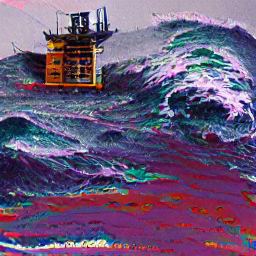
\includegraphics[width=.9\linewidth]{vqgan-images/vqgan-44}
}
%
What people think of when they hear the term \enquote{rogue wave} or \enquote{freak wave} heavily depends on their personal context, even among experts.

In popular science, the term rogue wave is often used to describe any large ocean wave, and they are often credited to be responsible for the loss of ships and lives at sea \citep{didenkulova_catalogue_2019}. This is contrary to the scientific definition, which is a relative criterion based on the observed wave height $H$ and the height of the surrounding waves, characterized by the significant wave height $H_s$:

\begin{align}
    \text{\footnotesize\spacedlowsmallcaps{Rogue wave criterion}} && \frac{H}{H_s} > \kappa && \label{eq:rogue}
\end{align}

Usually, the rogue threshold $\kappa$ is taken to be $2.0$ or $2.2$ for crest-to-trough wave heights and $1.2$ for crest heights. The significant wave height $H_s$ is defined as 4 times the standard deviation of the surface elevation (see \figref{fig:anatomy} for an illustration of these quantities). This is roughly equivalent to the mean of the highest third of waves, which aligns with the average wave height reported by a trained observer \citep{holthuijsen_waves_2010}.

\begin{figure}
    \begin{sidecaption}{Anatomy of an Eulerian wave observation, in which the observer is fixed in space (like a seaward facing laser, or --- approximately --- a tightly moored wave buoy).}[fig:anatomy]
		\antimpjustification
		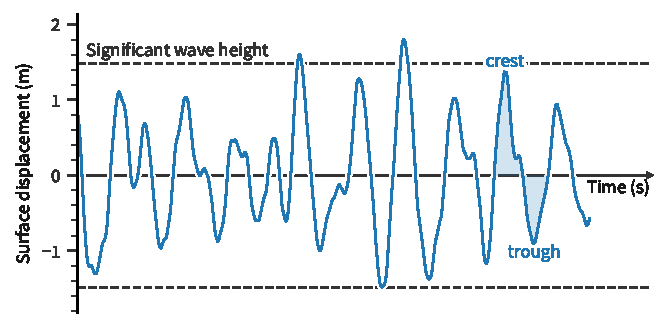
\includegraphics{sota/timeseries.pdf}
	\end{sidecaption}
\end{figure}

The definition \eqref{eq:rogue} immediately reveals the first fundamental issue in rogue wave research: most rogue waves are neither dangerous nor interesting. It is not noteworthy when a \SI{50}{\centi\metre} wave occurs in a \SI{20}{\centi\metre} sea state, but it is as much a rogue wave as a \SI{20}{\metre} wave in an \SI{8}{\metre} sea. For this definition to make sense, it implicitly encodes 2 fundamental assumptions:

\begin{enumerate}
    \item Small rogue waves are caused by the same generation mechanisms as big rogue waves.
    \item Waves above the rogue wave threshold are somehow fundamentally different from those below it.
\end{enumerate}

Both assumptions are non-trivial. In fact, the articles in \chapref{chap:main} present evidence that the second assumption does not hold throughout most sea states in the real ocean, and \chapref{chap:outro} discusses some of the implications.

Research interest in rogue waves was originally triggered by the indisputable measurement of a rogue wave at the Draupner oil rig in the North Sea in 1995, at a wave height of \SI{25.6}{\metre} and crest height of \SI{18.5}{\metre} during a storm with significant wave height of \SI{12}{\metre} \citep{sunde1995kjempebolger,haver2004possible}. With a relative crest height of \num{1.55}, this event would be extremely rare under the existing theory for linear, narrow-bandwidth waves \citep{longuet1952statisticaldistribution}. This disconnect sent the research community searching for a theory that attaches a higher probability to this and similar events.

This ultimately resulted in a debate on the fundamental nature of these waves: are they themselves extremely rare, or the conditions under which they are generated? Or in the words of \citeauthor{hayer2000freak}: \citebook{hayer2000freak}\sidenote[-4]{This is in fact an excellent question to address with machine learning. All we need to do is to see how well a model can reliably predict rogue waves given the sea state --- and hope that we have collected enough and the right kind of data.}. The following sections outline the ideas behind both hypotheses, and present the state of the art in rogue wave research.

\subsection{Linear Waves} \label{sec:waves-linear}

To lowest order, the properties of a 1-dimensional wave measurement (like a time series observation at a fixed location) are fully described by its spectral density $\mathcal{S}(f)$, often just called a \enquote{wave spectrum} (see \figref{fig:spectrum} for an example).

\begin{figure}
    \strictpagechecktrue
    \begin{sidecaption}{A typical bi-modal wave spectrum representing the overlap of swell and wind sea. Idealized Ochi-Hubble six-parameter wave spectrum with spectral peaks at periods \SI{6}{\second} and \SI{14}{\second} \citep{ochi_michel_k_six-parameter_1976}.}[fig:spectrum]
		\antimpjustification
		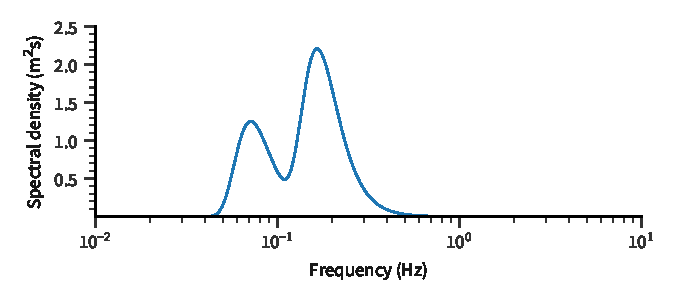
\includegraphics{sota/spectrum.pdf}
	\end{sidecaption}
\end{figure}

To see this, we adopt a simple model called the random phase-amplitude model \citep[see \eg][]{holthuijsen_waves_2010}: We view the wave train as a superposition of independent harmonics with frequency $f$, where each harmonic has an amplitude depending on the corresponding value of the wave spectrum $\mathcal{S}(f)$ and an independent, uniformly random phase $\phi \in (0, 2\pi)$. After all, many processes acting on waves in the real ocean are highly stochastic --- like wave generation from winds or scattering and refraction at a fractal coastline geometry --- so a random phase without a preferred value makes intuitive sense. In this case, the surface elevation $\eta$ is just the sum of each harmonic:

\begin{equation}
    \eta(t) = \sum_i \sqrt{2 \Delta f \mathcal{S}(f_i)} \sin(2\pi f_i t + \phi_i)
\end{equation}

\sidefigure{An ensemble of sea surface elevations drawn from the same wave spectrum (as shown in \figref{fig:spectrum}).}[fig:ensemble]{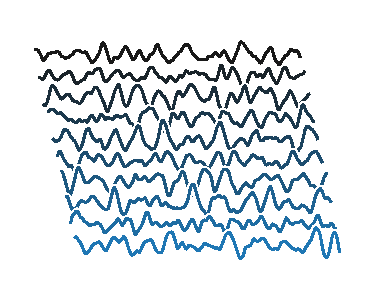
\includegraphics[width=\linewidth]{sota/ensemble.pdf}}[-1]
%
with time $t$, frequency $f$, frequency resolution $\Delta f$, and random phase $\phi$. In the case of a spectrum with many independent harmonics $f_i$ (as in the real ocean), this represents the sum of a large number of random variables with finite mean and variance. So per the central limit theorem, $\eta$ is a Gaussian random variable with zero mean and a variance that is fully determined by the significant wave height. This inherent stochasticity of random phases also implies that even under an identical spectrum no two wave fields will look exactly the same (\figref{fig:ensemble}).

In the limit of a narrow-band spectrum, the sea surface elevation only has one maximum / minimum per wave, and the wave heights and crest heights are Rayleigh distributed \citep{longuet1952statisticaldistribution,holthuijsen_waves_2010}:

\sidedef{Rayleigh wave distribution}{}{
\begin{align}
    \text{\footnotesize\spacedlowsmallcaps{Wave heights}} & & P(H / H_s > \kappa) &= \exp( -2 \kappa^2 ) \label{eq:rayleigh} \\
    \text{\footnotesize\spacedlowsmallcaps{Crest heights}} & & P(h / H_s > \kappa) &= \exp( -8 \kappa^2 )
\end{align}
}

These probability distributions will serve as the baseline for all further comparisons. They also tells us that, under these assumptions\sidenote[-1]{Assumptions behind Rayleigh-distributed wave heights:
\begin{renum}
    \item independent, non-interacting harmonics (linear waves);
    \item narrow spectral bandwidth.
\end{renum}
}, we would expect about \num{1} in \num{10000} waves to be a rogue wave (with a threshold $\kappa=2.0$ for waves and $1.2$ for crests) through mere random linear superposition.

Unfortunately, the real ocean is not so simple. One commonly violated assumption is that of \emph{narrow bandwidth}, which is used to derive the Rayleigh wave height distribution above. In fact, most seas do \emph{not} have Rayleigh distributed wave heights, as we will see in \chapref{chap:main} (not even seas that are approximately Gaussian). In particular, to create a rogue wave, both crest and trough have to be large, which makes them sensitive to the group structure of the wave train.

\sidefigure{Wave height probability density (top) and survival function for large wave heights (bottom). Curves are Tayfun distributions as in \eqref{eq:tayfun} with different values of $r$. The case $r=1$ is identical to the Rayleigh distribution \eqref{eq:rayleigh}.}[fig:wavedist]{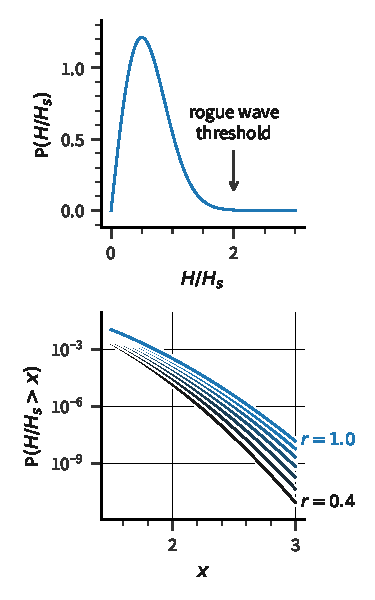
\includegraphics[width=\linewidth]{sota/wavedist.pdf}}
%
When taking finite bandwidths into account, things are more difficult, and there are several competing wave height distributions in bandwidth-limited seas \citep[\eg the Boccotti, Naess, and Tayfun distributions:][]{naess_distribution_1985,boccotti_mechanics_1989,tayfun_m._aziz_distribution_1990}. As an example, the Tayfun distribution is based on a parameter $r$ (which we call \emph{crest-trough correlation}) that is the value of the wave envelope at half the zero-crossing period (\ie at the expected location of the trough following a crest). For large wave heights $\gtrsim H_s$ it can be approximated as \citep{tayfun_wave-height_2007}:

\begin{equation}
    P(H / H_s > \kappa) = \sqrt{\frac{1 + r}{2 r}} \bigg( 1 + \frac{1-r^2}{4r\kappa^2} \bigg) \exp\bigg( -\frac{1}{4(1+r)} \kappa^2 \bigg) \label{eq:tayfun}
\end{equation}

with $r \in [0, 1]$. In the limit $r \to 1$ this reduces to the Rayleigh distribution for wave heights (\figref{fig:wavedist}).

\subsection{The Stokes Wave}

So far we have only considered waves and crests with independently random phases. This assumption is not fulfilled anymore as soon as waves are allowed to interact with each other, which couples the phases of different harmonics. Stokes theory extends this to weakly nonlinear waves with low characteristic steepness $\varepsilon = k H$ (with wave number $k$).

As in virtually all problems in fluid dynamics, an appropriate starting point is with the incompressible Navier-Stokes equations and the continuity equation (encoding momentum balance and mass conservation, respectively):

\sidedef{Navier-Stokes equations}{}{
\begin{gather}
\frac{\partial \vec{u}}{\partial t} + (\vec{u} \cdot \nabla) \vec{u} - \nu \nabla^2 \vec{u} = -\frac{1}{\rho} \nabla p - g \cdot \hat{k} \\
\nabla \cdot \vec{u} = 0
\end{gather}
}

with velocity vector $\vec{u}$, viscosity $\nu$, pressure $p$, density $\rho$, gravitational acceleration $g$, and unity vector in $z$ direction $\hat{k}$.

Assuming inviscid ($\nu=0$) and irrotational ($\nabla \times \vec{u} = 0$) fluid flow, we can introduce a velocity potential $\phi$:

\sidedef{Velocity potential}{}{
\begin{equation}
    \nabla \phi = \vec{u}
\end{equation}
}

This reduces the Navier-Stokes equations to the Bernoulli equation, and the continuity equation to a Laplace equation \citep[see \eg][]{holthuijsen_waves_2010}:

\sidedef{Bernoulli equation}{}{
\begin{gather}
\frac{\partial \phi}{\partial t} + \frac{1}{2} \lvert \nabla \phi
\rvert^2 \frac{p}{\rho} + gz = 0  \label{eq:bernoulli} \\
\nabla^2 \phi = 0
\end{gather}
}

A central missing ingredient is a set of boundary conditions at the top and bottom of the sea that give rise to finite surface elevations --- waves --- and shallow water effects. At each boundary we impose a kinematic boundary condition that ensures that water particles only move parallel to the respective surface $\eta(x, y, t)$:

\sidedef{Kinematic boundary condition}{}{
\begin{align}
    & u_z = \frac{\partial \eta}{\partial t} + u_x \frac{\partial \eta}{\partial x} + u_y \frac{\partial \eta}{\partial y} & \text{at $z=\eta$}\\
    \Leftrightarrow\quad & \frac{\partial\phi}{\partial z} = \frac{\partial \eta}{\partial t} + \frac{\partial \phi}{\partial x} \frac{\partial \eta}{\partial x} + \frac{\partial \phi}{\partial y} \frac{\partial \eta}{\partial y} & \text{at $z=\eta$} \label{eq:bc-kin}
\end{align}
}

For a flat bottom this just reduces to $\partial \phi / \partial z = 0$ at the ocean floor, but at the surface all terms are generally non-zero. At the surface we also find a dynamic boundary condition for the pressure $p$ that we plug into the Bernoulli equation:

\sidedef{Dynamic boundary condition}{}{
\begin{equation}
    p = 0 \quad\Rightarrow\quad \frac{\partial \phi}{\partial t} + \frac{1}{2} \lvert \nabla \phi \rvert^2 + g \eta = 0 \qquad \text{at $z=\eta$} \label{eq:bc-dyn}
\end{equation}
}

This assumes that the pressure at the water surface equals a constant atmospheric pressure.

The set of equations \eqref{eq:bernoulli}--\eqref{eq:bc-dyn} gives rise to a whole zoo of surface gravity waves in the ocean\sidenote[-1]{Excluding planetary-scale waves like Rossby and Kelvin waves, and neglecting interactions with bottom topograpy and breaking waves.}. The equations are nonlinear (containing terms $\propto \lvert \phi \rvert^2$ and $\nabla \phi \cdot \eta$) and cannot be solved analytically without further assumptions. The linear wave solution with non-interacting harmonics (as in \secref{sec:waves-linear}) is recovered by dropping all nonlinear terms and using the plane wave ansatz $\eta(x, t) = a \cos(\omega t - k x)$ with amplitude $a$, frequency $\omega$, and wave number $k$.

In the Stokes wave expansion, all nonlinear terms and unknown quantities (such as $\eta$ and $\omega$) are expanded in orders of the (assumed) small parameter $\varepsilon=ak$, the characteristic wave steepness \citep[see \eg][]{dean_water_1991}. By keeping only terms up to a certain order $n$ in $\varepsilon$, this leads to weakly nonlinear corrections of $n$-th order that generate wave trains with higher crests and flatter troughs than purely linear waves.

Weakly nonlinear corrections also cause a modification of the wave height distribution and enhance rogue wave probabilities, especially for rogue crests \citep{gemmrich_dynamical_2011,fedele_real_2016,fedele_large_2019}. This leads to conditions that have slightly elevated rogue wave probabilities, which supports the \enquote{rare realizations of a typical population} theory of rogue waves.

\subsection{Cnoidal Waves}

In shallow water the Stokes expansion converges very slowly, which makes Stokes theory inapplicable in this case (see \figref{fig:wave-regimes} for an overview). A characteristic parameter in this context is the Ursell number \citep{ursell_long-wave_1953}:

\sidedef{Ursell Number}{}{
\begin{equation}
    \mathrm{Ur} = \frac{\lambda^2 H}{D^3}
\end{equation}
}

with wavelength $\lambda = 2\pi/k$, wave height $H$, and water depth $D$. For high values of $\mathrm{Ur}$, an expansion in the relative depth $\widetilde{D}=kD$ is more fruitful than the Stokes expansion \citep{dean_water_1991}, which leads to the Korteweg-de Vries (KdV) equation and cnoidal theory \citep{korteweg1895xli}. Notably, cnoidal theory is the simplest theory that allows for solitary waves (solitons) --- waves that travel entirely above the water level and preserve their shape. Solitons have been studied intensely as a possible mechanism for rogue wave generation \citep{clamond_interaction_2002,kharif_physical_2003,chabchoub_rogue_2011}.

\begin{figure}
    \centering
    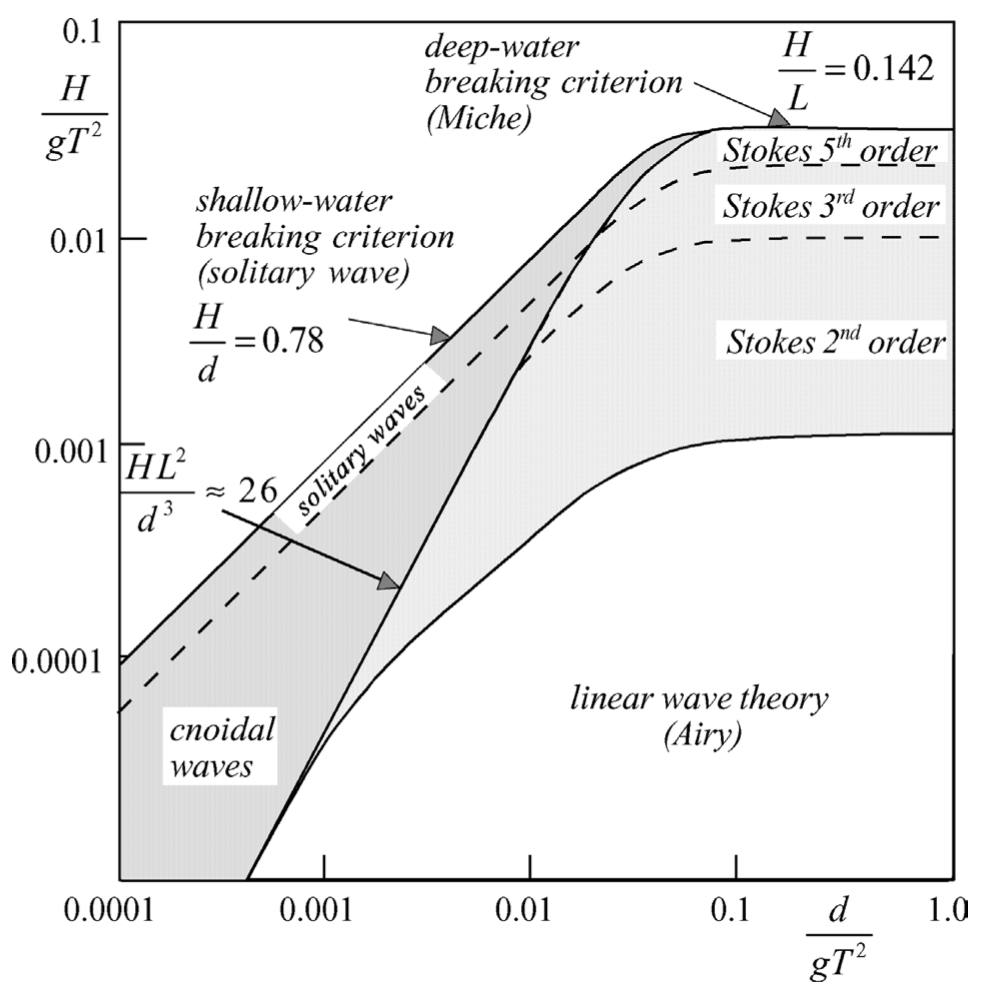
\includegraphics[width=.7\textwidth]{sota/wave-regimes.png}
    \caption{The range of applicability for different weakly nonlinear theories. From \citet{holthuijsen_waves_2010}, originally \citet{mehaute_introduction_2013}. Here, $T$ is the wave period, $H$ wave height, $d$ water depth, $L$ wavelength.} \label{fig:wave-regimes}
\end{figure}

\subsection{Highly Nonlinear Theory}

A large body of rogue wave research does not consider linear and weakly nonlinear solutions, as it is implicitly assumed that these mechanisms cannot be responsible for observed extreme rogue waves like the Draupner wave. Instead, these studies focus on highly nonlinear phenomena\sidenote[-3]{Highly nonlinear in the sense that these waves are not just small perturbations to the linear wave profile, but entirely new solutions with unique properties.} such as breathers, solitons, or the modulational instability as possible creation mechanisms \citep[\eg][]{kharif_physical_2003,onorato_extreme_2006,onorato_approximate_2012,toffoli_evolution_2010,shukla_instability_2006,kharif_focusing_2001,dematteis_experimental_2019}.

A prototypical framework for these solutions is the nonlinear Schrödinger equation (NLS), which is also based on an expansion in orders of characteristic steepness $\varepsilon$ and an expansion of the dispersion relation around a dominant wave number $k_0$ / frequency $\omega_0$ \citep[see \eg][for a derivation]{johnson_modern_1997}. In contrast to the Stokes wave solution, the (now complex) wave amplitude $A(x, t)$ is allowed to evolve in time and space and satisfies the nonlinear Schrödinger equation \citep{slunyaev_rogue_2011}:

\sidedef{Nonlinear Schrödinger equation}{}{
\begin{equation}
    -2i \bigg(\frac{\partial A}{\partial t} + c_g \frac{\partial A}{\partial x} \bigg) + \frac{\omega_0}{8 k_0^2} \frac{\partial^2 A}{\partial x^2} + \frac{\omega_0 k_0^2}{2} A \lvert A \rvert^2 = 0
\end{equation}
}

with group speed $c_g$. This equation has solutions that grow exponentially due to energy transfer between the carrier wave and its sidebands, an effect called modulational instability or Benjamin-Feir instablity \citep{benjamin_disintegration_1967}. These solutions are referred to as breathers, one of which is the Peregrine soliton \citep[\figref{fig:peregrine}]{peregrine_water_1983}. The strength of the modulational instability is governed by the Benjamin-Feir index \citep{alber_effects_1978}:
%
\sidefigure{The Peregrine solution. Shown is the evolution of the wave height envelope $A$ in space and time, with a clear localized maximum.}[fig:peregrine]{
    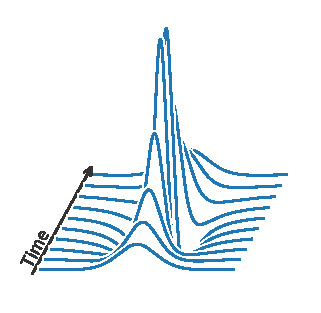
\includegraphics{sota/peregrine.pdf}
}[3.3]

\sidedef{Benjamin-Feir index}{}{
    \begin{equation}
        \mathrm{BFI} = \frac{k_0 A}{\Delta\omega / \omega_0}
    \end{equation}
}

with spectral bandwidth $\Delta \omega$. The original derivation of the nonlinear Schrödinger equation assumes deep water, unidirectional propagation, and narrow-banded spectra. Modifications that relax these assumptions exist \citep{davey_three-dimensional_1974,dysthe_note_1979}, and modified versions of the BFI that take shallow water and directional spreading into account have been suggested \citep{serio_computation_2005,fedele_kurtosis_2015}. There is good evidence demonstrating the modulational instability in wave tanks \citep{onorato_extreme_2006}, but studies considering real ocean conditions have so far not confirmed an enhancement of extreme waves \citep{gramstad_influence_2007,xiao_rogue_2013}.

The nonlinear Schrödinger equation is not the only nonlinear wave equation with unstable solutions. In general, waves transfer energy via nonlinear four-wave interactions \citep{hasselmann_feynman_1966}. This is accounted for explicitly in the Zakharov equation \citep{zakharov_stability_1968}, which can be studied to derive higher-order corrections to the wave height distribution \citep[\eg as in][]{janssen_nonlinear_2003}.

\subsection{Other Causes of Rogue Waves}

There are several other hypothesized causes for rogue waves that we have not considered so far \citep[see][for reviews]{adcock_physics_2014,slunyaev_rogue_2011,dudley_rogue_2019}. While the Bernoulli equations \eqref{eq:bernoulli} and associated boundary conditions are very general in terms of the permitted dynamics \emph{within} the fluid, most of the real-world complexities \emph{outside} the fluid are neglected. Examples for this include:

\begin{items}
    \item Interactions with non-uniform topography such as abrupt transitions in water depth or waves on top of a slope \citep{trulsen_laboratory_2012};
    \item The non-stationarity of the sea state, \ie its evolution in time \citep{trulsen_rogue_2018};
    \item The interaction between waves and currents \citep{mallory_abnormal_1974,didenkulova_rogue_2021,onorato_triggering_2011};
    \item Direct wind-wave interactions \citep{adcock_energy_2011};
    \item Wave breaking, \eg the influence of crossing seas on the onset and shape of breaking waves \citep{mcallister_laboratory_2019}.
\end{items}

All of these effects impact the formation of large waves, but they are also inherently \emph{local}, which causes them to be averaged out of bulk statistics (such as buoy measurements from many different locations).

\clearpage

\section{Physics and Machine Learning} \label{sec:sota-ml}

\sidefigure{AI art generated by VQGAN + CLIP \citep{esser_taming_2021,radford_learning_2021}. Prompt: \emph{\enquote{a cartoon robot surfing on a big wave}}.}{
    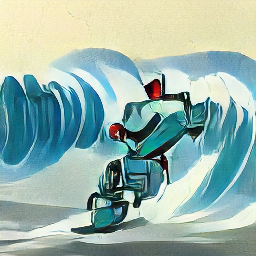
\includegraphics[width=.9\linewidth]{vqgan-images/vqgan-24.png}
}
%
The are many examples of studies that apply machine learning to physical problems, most of which aim for improvements in computational efficiency or predictive performance of simulations \citep[\eg][]{pestourie_physics-enhanced_2021,bar-sinai_data-driven_2018,kochkov_machine_2021,li_kohn-sham_2020,cranmer_bayesian_2021,cranmer_lagrangian_2020}.
These efforts undoubtedly contribute tremendous value. Yet, better \emph{predictions} are not the same as improved \emph{understanding}, the foundation of all science. Ideally, machine learning would lead to advances on both fronts, but unfortunately, process understanding seems much harder to come by, in part also due to the immense complexity of real-world data and governing processes \citep[\figref{fig:ml-challenges};][]{reichstein_deep_2019}.

\begin{figure}
    \begin{sidecaption}{Challenges when applying machine learning to earth system data. Figure from \citet{reichstein_deep_2019}.}[fig:ml-challenges]
        \antimpjustification
        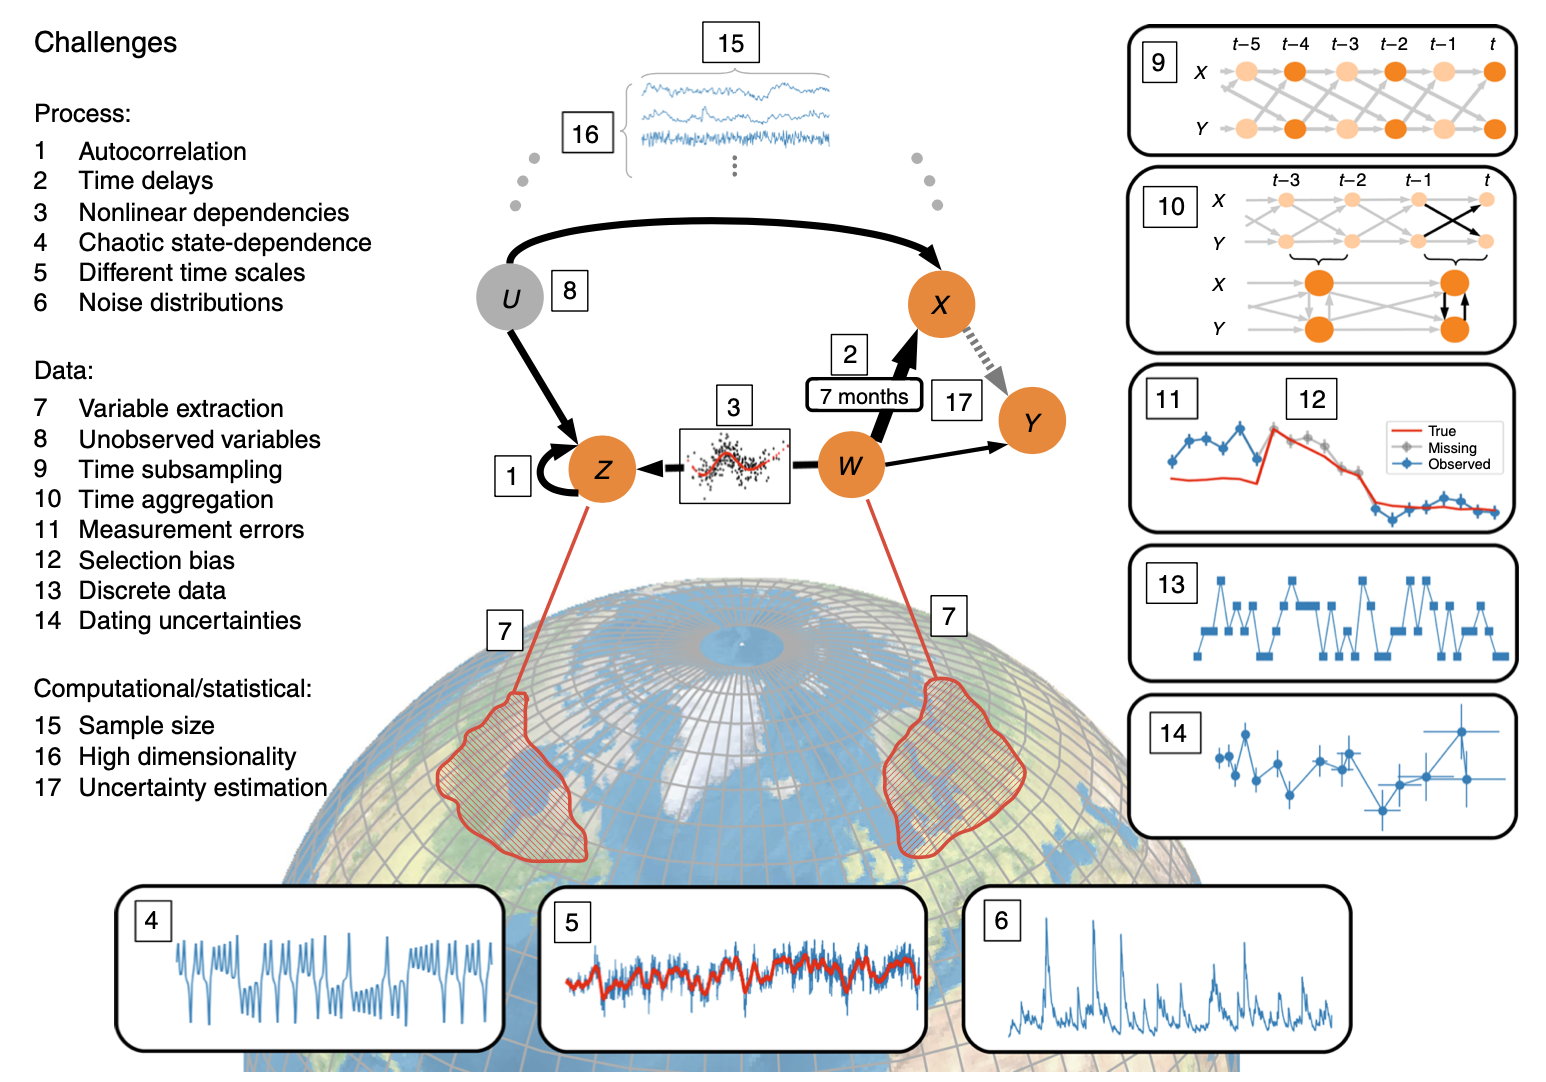
\includegraphics[width=\textwidth]{sota/ml-challenges.png}
    \end{sidecaption}
\end{figure}

One necessary ingredient for true understanding is the robust identification of causal connections over mere association. The emerging field of causality has formalized the identifiability of causal connections from data and provides tools for both causal inference and causal discovery \citep[see \eg][]{peters_elements_2017}. There are first promising applications of these methods \citep[for example in climate:][]{hannart_causal_2016,kretschmer_using_2016,runge_inferring_2019}, but it is still a long way to go before we will be able to identify arbitrary causal connections in real-world spatiotemporal systems. Nevertheless, explicitly encoding or enforcing causal relationships in models is a promising way to make machine learning a more dependable tool for scientific discovery.

Causal connections in physical systems are typically representable by simple mathematical relationships\sidenote[-1]{An observation dubbed \citebook{wigner_unreasonable_1960}.}. Machine learning can exploit this through symbolic regression, a method that aims to fit sparse mathematical expressions to data. While the idea itself is not new \citep[traditionally based on genetic programming,][]{schmidt_distilling_2009}, it is now elevated through increasingly sophisticated machine learning algorithms, with some first successes \citep{udrescu_ai_2020,zanna_data-driven_2020,lemos_rediscovering_2022,cranmer_discovering_2020}.

An in physics ubiquitous special case is systems of differential equations, which can be replaced or augmented with neural networks \citep[neural ODEs / UDEs,][]{chen_neural_2019,rackauckas_universal_2021,kidger_neural_2022}. In combination with symbolic regression, this leads to methods for the automated discovery of differential equations (and thus system dynamics) from data, an approach that shows huge potential \citep{brunton_discovering_2016,long_pde-net_2019,champion_data-driven_2019,bakarji_discovering_2022,reinbold_robust_2021} but is still very much a matter of active research, and still struggles with observational noise.
%
\sidefigure{The increasing resolution of climate models over time leads to exponentially increasing data volumes. Horizontal resolution over Europe from IPCC (Intergovernmental Panel on Climate Change) reports FAR (1990), SAR (1996), TAR (2001a), and AR4 (2007). Figure from \citet{change2007climate}.}[fig:climate-res]{
    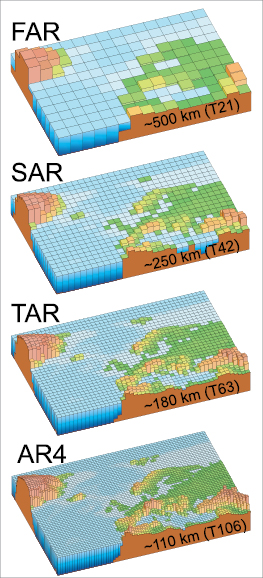
\includegraphics[width=.9\linewidth,trim=5 5 5 5,clip]{sota/climate-res.jpeg}
}[-12]

A methodologically much simpler approach is \enquote{data-mining inspired induction} \citep{voit_perspective_2019}, where interpretable machine learning \citep{molnar_interpretable_nodate} and data mining guide the scientist towards the formation of hypotheses that can then be independently verified --- as opposed to setting out with a specific hypothesis to test.

Data-mining inspired induction addresses a common challenge in modern science: data volumes have increased exponentially in the last decades (\figref{fig:climate-res}), while human resources are approximately fixed. The central idea is to combine the strengths of machine learning models (large-scale data analysis taking into account orders of magnitude more data than the human mind could) and humans (causal reasoning and interpretation) into a modern scientific workflow. The remainder of this thesis is a concrete application of this approach and serves as a case study on its feasibility, challenges, and opportunities on a real physical problem.
